\documentclass[12pt, a4paper]{article}

% ===== 패키지 =====
\usepackage{fontspec}         % XeLaTeX/LuaLaTeX 폰트 설정
\usepackage{kotex}            % 한글 지원
\usepackage{geometry}
\geometry{margin=2.5cm}
\usepackage{minted}           % 코드 삽입 (XeLaTeX + shell-escape 필요)
\usepackage{xcolor}           % 색상
\usepackage{booktabs}         % 깔끔한 표
\usepackage{amsmath, amssymb} % 수식
\usepackage{hyperref}         % 하이퍼링크
\usepackage{graphicx}         % 이미지
\usepackage{enumitem}         % 리스트 커스텀
\usepackage{caption}
\usepackage{adjustbox}        % 큰 표 너비 조절용
\usepackage{pifont}           % 체크마크 기호용
\usepackage[normalem]{ulem}   % 취소선 (\sout)
\newcommand{\cmark}{\ding{51}}
\usepackage{tikz}             % 순서도 도형
\usetikzlibrary{shapes.geometric, arrows.meta, positioning}

% ===== 코드 스타일 =====
\setminted[python]{
    bgcolor=black!5,
    linenos=true,
    breaklines=true,
    fontsize=\small,
    frame=lines,
    framesep=2mm
}

% ===== 문서 정보 =====
% 제목/저자 정보는 커스텀 헤더로 직접 구성

% ========================================
\begin{document}

% ===== 커스텀 헤더 (제목 페이지 없이 바로 시작) =====
\begin{center}
    {\Large\bfseries Programming Assignment \#2}\\[0.4em]
    {\large\bfseries 의사결정 나무(Decision Tree) 분류기 구현}\\[1em]
    {\normalsize
        \textbf{과목:} Data Science (ITE4005) \quad
        \textbf{학번:} 2023036299 \quad
        \textbf{이름:} 김진욱 \quad
        \textbf{2026.04.03}\\[0.3em]
        \textbf{OS:} Windows 10/11 \quad
        \textbf{Python:} 3.12.10 \quad
        \textbf{라이브러리:} 표준 라이브러리 (\texttt{sys}, \texttt{math}, \texttt{collections})
    }
\end{center}
\vspace{0.5em}
\hrule
\vspace{1em}

% ============================================================
\section{과제 핵심 요구사항 요약}
% ============================================================

\begin{itemize}
    \item \textbf{프로그램 형식}: 파이썬 스크립트(\texttt{dt.py})로 구현하며, 터미널(CMD) 환경에서 실행.
    \item \textbf{실행 명령어}: \texttt{python dt.py dt\_train.txt dt\_test.txt dt\_result.txt} (명령어 인자 3개 필수)
    \item \textbf{파일 위치}: 스크립트, train, test, result 파일은 모두 동일한 폴더(동일 경로)에 위치해야 함.
    \item \textbf{출력 규격}:
    \begin{itemize}
        \item 결과 파일의 각 데이터 값은 반드시 탭(\texttt{\textbackslash t})으로 구분할 것.
        \item 테스트 셋의 원래 데이터 행 순서를 절대 변경하지 말 것.
        \item 결과의 첫 행은 기존 속성 이름들 맨 뒤에 테스트 할 `클래스 라벨(정답열 이름)'을 추가할 것.
        \item 결과의 나머지 행들은 기존 테스트 데이터 맨 뒤에 탭(\texttt{\textbackslash t})과 함께 트리가 `결정한 예측값'을 추가할 것.
    \end{itemize}
\end{itemize}


% ============================================================
\section{입출력 데이터 형태 분석}
% ============================================================

\texttt{dt\_train.txt}(학습), \texttt{dt\_test.txt}(시험), \texttt{dt\_answer.txt}(기대 결과)를 분석하여 다음과 같은 구현 워크플로우를 도출했다.

\begin{enumerate}
    \item \textbf{Train (학습)}
    \begin{itemize}
        \item 데이터 파일의 첫 줄에서 속성 이름들을 파악하고, 마지막 열의 속성(예: \texttt{Class:buys\_computer})을 분류해야 할 Target 변수(정답)로 설정한다.
        \item \texttt{dt\_train.txt}를 읽고 Info Gain 등의 척도를 계산하여 트리를 훈련시킨다.
    \end{itemize}
    \item \textbf{Test (예측) \& Export (출력)}
    \begin{itemize}
        \item \texttt{dt\_test.txt}는 정답열 없이 주어진다. 이를 훈련된 트리에 통과시켜 각 행의 정답을 추론한다.
        \item 원본 테스트 데이터를 그대로 하나씩 출력 파일에 기록하되, 각 줄의 맨 끝에 모델이 추론한 값을 덧붙여서 기록한다.
    \end{itemize}
\end{enumerate}


% ============================================================
\section{핵심 알고리즘 (연속형 변수 처리 관련)}
% ============================================================

\begin{itemize}
    \item \textbf{분할 기준 (Split Criterion)}:
    Information Gain, Gain Ratio, Gini Index 중 하나를 수식으로 구현하여 어떤 속성(Attribute)으로 트리의 노드(Branch)를 나눌지 결정한다.

    \item \textbf{연속형 데이터(Threshold) 계산 시 주의점}:
    \begin{itemize}
        \item 과제 지시문에 기반하여, 본 모델은 \textbf{오직 범주형(Categorical) 데이터만 취급}한다.
        \item \texttt{age} 속성에 포함된 \texttt{<=30}, \texttt{31...40}, \texttt{>40} 같은 값들은 부등호나 숫자로 보이더라도 대소로 분리해야 할 ``연속된 숫자의 범위''로 해석할 필요가 없다.
        \item 컴퓨터 입장에서는 이를 \texttt{income}의 \texttt{high}, \texttt{low}와 완벽하게 동일한 \textbf{고유 텍스트 카테고리(일반 문자열)}로 취급하면 된다.
        \item 따라서 코드를 짤 때 숫자의 대소비교나 임계값(Threshold)을 계산해 이분할(Binary Split)하는 로직은 필요하지 않으며, 데이터상에 존재하는 고유한 글자들의 종류(Unique values)대로 곧바로 자연스러운 N갈래 가지치기를 진행하면 된다.
    \end{itemize}
\end{itemize}


% ============================================================
\section{고급 분할 전략 (동점 및 Bias 처리 로직)}
% ============================================================

보고서(Report) 작성 시 알고리즘의 우수성을 돋보이게 할 수 있는 \textbf{앙상블(혼합) 분할 척도 전략}에 대한 아이디어이다.

\begin{itemize}
    \item \textbf{Information Gain의 치명적 한계점}:
    고유한 값이 매우 많아 데이터가 무수히 잘게 쪼개지는 속성을 `가장 좋은 속성'으로 착각하는 편향(Bias) 문제가 있다.
    (참고: 이를 이론적으로 해결하기 위해 `잘게 쪼개는 것'에 페널티(Split Info)를 주는 수식인 Gain Ratio가 C4.5 알고리즘에서 고안되었다.)

    \item \textbf{혼합(Hybrid) 전략 아이디어 적용 방안}:
    \begin{enumerate}
        \item 구현이 가장 직관적이고 널리 쓰이는 \textbf{Information Gain}을 기본(Default) 분기 엔진으로 장착한다.
        \item 트리가 깊어지거나 데이터가 적어 여러 속성의 \textbf{Information Gain 수치가 소수점까지 동일한 동점(Tie)} 상황이 발생했을 경우, 임의로 아무 속성을 고르지 않고 보조 엔진으로 \textbf{Gain Ratio (또는 Gini Index)를 계산하여 승자를 판가름(Tie-breaker)}한다.
        \item 이러한 예외 처리(Exception handling) 방식을 추가한다면 모델의 안정성과 정교함을 끌어올릴 수 있으며, 추후 보고서 작성 시 높은 점수를 얻기 위한 매우 훌륭한 차별화 요소가 될 수 있다.
    \end{enumerate}
\end{itemize}


% ============================================================
\section{구현 완료 --- 각 함수별 설계 철학 및 Python 기능 선택 근거}
% ============================================================

\subsection{전체 프로그램 구조 (파이프라인)}

\begin{figure}[h]
\centering
\begin{tikzpicture}[
    node distance=0.75cm and 2cm,
    box/.style={rectangle, rounded corners=5pt, draw=black!70, fill=blue!8,
                minimum width=8cm, minimum height=0.8cm,
                align=center, font=\small},
    loopbox/.style={rectangle, rounded corners=5pt, draw=black!60, fill=orange!10,
                    minimum width=8cm, minimum height=1.6cm,
                    align=center, font=\small},
    arr/.style={->, thick, draw=black!60}
]
\node[box] (start)    {시작};
\node[box, below=of start]   (read)    {\texttt{read\_data()} \\ 데이터 읽기};
\node[box, below=of read]    (split)   {\texttt{header[-1]} = target, \texttt{header[:-1]} = features \\ 타겟/피처 분리};
\node[loopbox, below=of split] (build) {\texttt{build\_tree()} $\leftarrow$ 재귀 호출 \\
    \texttt{select\_best\_attribute()} \\
    \texttt{information\_gain()} $\leftarrow$ 1차 기준 $\cdot$ \texttt{entropy()} \\
    \texttt{gain\_ratio()} $\leftarrow$ 동점 시 보조 기준 $\cdot$ \texttt{split\_info()}};
\node[box, below=of build]   (pred)    {\texttt{predict\_all()} $\to$ \texttt{predict\_one()} $\leftarrow$ 재귀 호출 \\ 테스트 데이터 예측};
\node[box, below=of pred]    (write)   {\texttt{write\_result()} \\ 결과 파일 저장};
\node[box, below=of write]   (end)     {종료};

\draw[arr] (start)  -- (read);
\draw[arr] (read)   -- (split);
\draw[arr] (split)  -- (build);
\draw[arr] (build)  -- (pred);
\draw[arr] (pred)   -- (write);
\draw[arr] (write)  -- (end);
\end{tikzpicture}
\caption{의사결정 나무 분류기 전체 파이프라인}
\end{figure}


\subsection{\texttt{read\_data()} --- 데이터 파싱의 핵심 설계}

\begin{minted}{python}
row = dict(zip(header, values))
\end{minted}

\noindent\textbf{\texttt{dict(zip(header, values))} 선택 이유:}
\begin{itemize}
    \item 각 데이터 행을 \texttt{\{속성이름: 값\}} 형태의 딕셔너리로 변환한다.
    \item 이를 통해 코드 전체에서 \texttt{row['age']}, \texttt{row['buying']} 처럼 \textbf{속성 `이름'으로} 값에 접근할 수 있다.
    \item 인덱스 번호(\texttt{row[0]}, \texttt{row[2]}) 대신 이름을 쓰기 때문에, 속성 이름이 \texttt{buys\_computer}에서 \texttt{car\_evaluation}으로 바뀌어도 코드 수정이 전혀 필요 없다.
    \item 이것이 \textbf{``하드코딩 없는 범용성''}의 핵심 설계이다.
\end{itemize}


\subsection{\texttt{entropy()} --- 엔트로피 계산}

\begin{minted}{python}
labels = [row[target] for row in data]
counts = Counter(labels)
\end{minted}

\noindent\textbf{\texttt{collections.Counter} 선택 이유:}
\begin{itemize}
    \item 리스트의 각 원소가 몇 번 등장하는지를 \textbf{한 번의 순회($O(n)$)}로 딕셔너리 형태로 집계해준다.
    \item 수동 \texttt{for문 + if문 + dict} 카운팅 방식보다 간결하고 Pythonic하다.
    \item $p = 0$일 때 $\log_2(0)$은 수학적으로 정의 불가이므로, $p > 0$ 조건으로 건너뛴다 ($\lim_{p \to 0} p \log_2 p = 0$이므로 수학적으로도 올바른 처리).
\end{itemize}


\subsection{\texttt{information\_gain()} --- 정보 이득 계산의 효율성}

\begin{minted}{python}
partitions = {}
for row in data:
    val = row[attribute]
    if val not in partitions:
        partitions[val] = []
    partitions[val].append(row)
\end{minted}

\noindent\textbf{명시적 for문 그룹핑 선택 이유:}
\begin{itemize}
    \item 리스트 컴프리헨션으로 속성값별 필터링을 하면 (\texttt{[row for row in data if row[attr] == v]}), 고유값이 $k$개일 때 \textbf{데이터를 $k$번 순회($O(n \times k)$)}한다.
    \item 반면 위 방식은 \textbf{한 번의 순회($O(n)$)}로 모든 그룹핑이 완료된다.
    \item 대규모 데이터셋(\texttt{dt\_train1.txt}, 1383행)에서 이 차이가 체감 성능에 영향을 준다.
\end{itemize}


\subsection{\texttt{split\_info()} \& \texttt{gain\_ratio()} --- 보조 분할 척도}

\begin{itemize}
    \item \texttt{split\_info()}의 수식 구조는 \texttt{entropy()}와 동일하지만, `클래스 라벨'이 아닌 \textbf{`속성값'의 분포}를 기준으로 계산한다는 차이가 있다. 함수를 분리하여 이 의미적 차이를 명확히 했다.
    \item \texttt{gain\_ratio()}에서 Split Information이 0인 경우(모든 데이터가 같은 속성값) $\to$ 0으로 나누기 방지를 위해 \texttt{0.0}을 반환한다.
\end{itemize}


\subsection{\texttt{select\_best\_attribute()} --- 혼합(Hybrid) 전략 구현}

\begin{minted}{python}
# 1차: Information Gain으로 동점 후보를 모은다
for attr in attributes:
    ig = information_gain(data, attr, target)
    if ig > best_gain:
        best_gain = ig
        candidates = [attr]
    elif ig == best_gain:
        candidates.append(attr)

# 2차: 동점이면 Gain Ratio로 승부
if len(candidates) == 1:
    return candidates[0]
best_attr = max(candidates, key=lambda attr: gain_ratio(data, attr, target))
\end{minted}

\noindent\textbf{\texttt{max()} + \texttt{key=lambda} 선택 이유:}
\begin{itemize}
    \item \texttt{max(iterable, key=func)}는 \texttt{func}의 반환값이 최대인 원소를 $O(n)$에 찾아준다.
    \item 수동 for문으로 최대값과 그 인덱스를 동시에 추적하는 것보다 간결하다.
\end{itemize}

\noindent\textbf{동점 후보를 리스트로 모으는 이유:}
\begin{itemize}
    \item 단순히 \texttt{max(attributes, key=ig\_func)}를 쓰면 동점 시 첫 번째 원소가 자동 선택되어, Tie-breaker 로직을 삽입할 여지가 없다.
\end{itemize}


\subsection{\texttt{build\_tree()} --- 트리를 중첩 딕셔너리(nested dict)로 표현}

\begin{minted}{python}
tree = {best_attr: {}}
# 예시 결과:
# {'age': {'<=30': {'student': {'yes': 'yes', 'no': 'no'}},
#          '31...40': 'yes',
#          '>40': {'credit_rating': {'fair': 'yes', 'excellent': 'no'}}}}
\end{minted}

\noindent\textbf{별도 Node 클래스 대신 dict를 선택한 이유:}
\begin{itemize}
    \item 클래스 정의 없이도 트리를 자연스럽게 표현 가능.
    \item \texttt{print(tree)}로 즉시 구조를 확인할 수 있어 디버깅이 용이.
    \item dict의 key가 속성값(branch), value가 자식 노드(subtree) 또는 리프 노드(문자열 라벨).
\end{itemize}

\noindent\textbf{재귀 종료 조건 3가지:}
\begin{enumerate}
    \item \textbf{모든 클래스가 동일} $\to$ \texttt{set()}으로 고유 라벨을 추출, 1개면 리프.
    \item \textbf{남은 속성이 없음} $\to$ \texttt{Counter.most\_common(1)}로 다수결 리프.
    \item \textbf{데이터가 비어있음} $\to$ 상위 호출의 \texttt{majority\_label} 사용.
\end{enumerate}

\noindent\textbf{\texttt{Counter.most\_common(1)} 선택 이유}: 최빈값을 $O(n)$에 찾아준다. \texttt{sorted() + [0]} 방식보다 의도가 명확하고 효율적이다.


\subsection{\texttt{predict\_one()} --- 타입 기반 노드 구분}

\begin{minted}{python}
if not isinstance(tree, dict):
    return tree  # str이면 리프 노드
attr_name = list(tree.keys())[0]  # dict면 내부 노드
\end{minted}

\noindent\textbf{\texttt{isinstance(tree, dict)} 선택 이유:}
\begin{itemize}
    \item 트리를 dict로 표현했기 때문에, 타입 자체가 노드 종류를 결정한다.
    \item \texttt{dict}이면 아직 내부 노드 $\to$ 속성값에 따라 하위로 이동.
    \item \texttt{str}이면 리프 노드 $\to$ 해당 문자열이 예측 결과.
\end{itemize}

\noindent\textbf{예외 처리 --- 학습 데이터에 없던 속성값:}
테스트에 학습 시 본 적 없는 속성값이 등장할 수 있으므로, \texttt{default\_label}(전체 학습 데이터의 다수결 라벨)을 반환한다.


\subsection{\texttt{predict\_all()} --- 리스트 컴프리헨션의 활용}

\begin{minted}{python}
return [predict_one(tree, row, default_label) for row in test_data]
\end{minted}

\noindent\textbf{리스트 컴프리헨션 선택 이유:}
\begin{itemize}
    \item \texttt{for문 + append}보다 Pythonic하고, 내부적으로 C 레벨 최적화가 적용되어 약간 더 빠르다.
    \item 입력 순서가 그대로 유지되므로, ``테스트 데이터의 행 순서를 변경하지 말 것'' 과제 요구사항을 자연스럽게 충족한다.
\end{itemize}


% ============================================================
\section{1차 테스트 결과}
% ============================================================

\subsection{소규모 데이터셋 (buys\_computer)}

\begin{table}[h]
\centering
\begin{adjustbox}{max width=\textwidth}
\begin{tabular}{ll}
\toprule
\textbf{항목} & \textbf{값} \\
\midrule
학습 데이터   & \texttt{dt\_train.txt} (14행) \\
테스트 데이터 & \texttt{dt\_test.txt} (5행) \\
정답 파일     & \texttt{dt\_answer.txt} \\
\textbf{정확도} & \textbf{5/5 = 100\%} \cmark \\
\bottomrule
\end{tabular}
\end{adjustbox}
\caption{소규모 데이터셋 테스트 결과}
\end{table}

출력 파일(\texttt{dt\_result.txt})이 정답 파일(\texttt{dt\_answer.txt})과 \textbf{바이트 단위로 완벽 일치}했다.

\subsection{대규모 데이터셋 (car\_evaluation)}

\begin{table}[h]
\centering
\begin{adjustbox}{max width=\textwidth}
\begin{tabular}{ll}
\toprule
\textbf{항목} & \textbf{값} \\
\midrule
학습 데이터   & \texttt{dt\_train1.txt} (1383행, 6개 속성) \\
테스트 데이터 & \texttt{dt\_test1.txt} (346행) \\
정답 파일     & \texttt{dt\_answer1.txt} \\
\textbf{정확도} & \textbf{303/346 = 87.57\%} \\
\bottomrule
\end{tabular}
\end{adjustbox}
\caption{대규모 데이터셋 테스트 결과}
\end{table}

\begin{itemize}
    \item 42건의 불일치가 발생했다.
    \item 의사결정 나무의 오버피팅(Overfitting) 특성상, 학습 데이터에 과적합된 트리가 테스트 데이터의 일부 패턴을 놓치는 것은 자연스러운 현상이다.
\end{itemize}

\subsection{범용성 검증}

\begin{itemize}
    \item \textbf{동일한 코드(\texttt{dt.py})} 하나로 \texttt{buys\_computer} 데이터셋과 \texttt{car\_evaluation} 데이터셋 모두를 정상적으로 처리하였다.
    \item 속성 이름, 속성 개수, 클래스 라벨의 종류가 완전히 달라도 코드 수정 없이 동작함을 확인 $\to$ \textbf{하드코딩 없는 범용 설계 검증 완료}.
\end{itemize}


% ============================================================
\section{분할 기준 비교 실험 (A / B / C)}
% ============================================================

\subsection{실험 배경}

정답 파일이 \textbf{어떤 분할 기준으로 생성되었느냐}에 따라 트리의 모양이 달라질 수 있으므로,
분할 기준을 바꿔가며 정확도가 개선되는지 비교 실험을 수행하였다.

\subsection{실험별 변경 내용}

\begin{table}[h]
\centering
\begin{adjustbox}{max width=\textwidth}
\begin{tabular}{lllp{6cm}}
\toprule
\textbf{실험} & \textbf{1차 기준} & \textbf{동점 해소} & \textbf{핵심 코드} \\
\midrule
기존   & Info Gain        & Gain Ratio   & \texttt{max(candidates, key=gain\_ratio)} \\
A      & Gain Ratio 단독  & ---          & \texttt{max(attrs, key=gain\_ratio)} \\
B      & Gini Index 단독  & ---          & \texttt{min(attrs, key=gini\_index)} \\
C      & Gain Ratio       & Gini Index   & \texttt{min(candidates, key=gini\_index)} \\
\bottomrule
\end{tabular}
\end{adjustbox}
\caption{실험별 분할 기준 변경 내용}
\end{table}


% ============================================================
\section{정밀 재검증 --- 단일 스크립트 동시 비교}
% ============================================================

\subsection{재검증 배경}

실험 A, B, C의 결과가 모두 동일(87.57\%)하게 나와 \textbf{``파일 변경이 제대로 반영되지 않은 채 실험을 돌린 것이 아닌가?''}라는 의심이 제기되었다.

\subsection{재검증 방법}

의심을 해소하기 위해, \textbf{하나의 Python 스크립트 내에서 4가지 전략 함수를 정의하고 동시에 실행}하여 파일 저장/반영 문제를 완전히 배제한 정밀 검증을 수행하였다.

\begin{minted}{python}
# 단일 프로세스에서 4가지 전략을 동시에 비교
for name, select_fn in [('IG+GR_tie', s1), ('GR_only', s2),
                         ('Gini_only', s3), ('GR+Gini_tie', s4)]:
    tree = build_tree_custom(train, features, target, select_fn)
    preds = [predict_one(tree, row, default) for row in test]
    match = sum(1 for i in range(len(preds)) if preds[i] == answer[i])
    print(f'{name}: {match}/{len(preds)} = {match/len(preds)*100:.2f}%')
\end{minted}

\subsection{재검증 결과}

\begin{verbatim}
IG+GR_tie:   303/346 = 87.57%
GR_only:     303/346 = 87.57%
Gini_only:   303/346 = 87.57%
GR+Gini_tie: 303/346 = 87.57%
\end{verbatim}

\textbf{4가지 전략이 코드 변경이 정확히 반영된 상태에서도 완벽히 동일한 결과를 냄을 확인하였다.}


% ============================================================
\section{전체 실험 종합 비교}
% ============================================================

\begin{table}[h]
\centering
\begin{adjustbox}{max width=\textwidth}
\begin{tabular}{llll}
\toprule
\textbf{\#} & \textbf{분할 기준} & \textbf{buys\_computer} & \textbf{car\_evaluation} \\
\midrule
기존   & Info Gain + Gain Ratio Tie-break       & 100\% & 87.57\% \\
실험 A & Gain Ratio 단독                        & 100\% & 87.57\% \\
실험 B & Gini Index 단독                        & 100\% & 87.57\% \\
실험 C & Gain Ratio + Gini Index Tie-break      & 100\% & 87.57\% \\
\bottomrule
\end{tabular}
\end{adjustbox}
\caption{전체 실험 종합 비교}
\end{table}

\subsection{종합 분석 --- 왜 4가지 전략이 모두 동일한 결과를 내는가?}

\begin{itemize}
    \item \textbf{근본 원인}: car\_evaluation 데이터셋의 6개 속성(\texttt{buying}, \texttt{maint}, \texttt{doors}, \texttt{persons}, \texttt{lug\_boot}, \texttt{safety})이 모두 \textbf{3\textasciitilde4개의 매우 비슷한 고유값 개수}를 가지고 있다.
    \begin{itemize}
        \item 이 경우 Information Gain, Gain Ratio, Gini Index가 \textbf{대부분의 노드에서 동일한 속성을 최적으로 선택}한다.
        \item 고유값 개수가 균등하면 Split Information(분할 정보량)의 보정 효과가 거의 없으므로, Gain Ratio $\approx$ Information Gain이 된다.
        \item 마찬가지로 Gini Index도 엔트로피 기반 척도와 유사한 순위를 매기게 된다.
        \item 결과적으로 \textbf{4가지 전략 모두 동일한 트리를 생성}하여 예측 결과가 같아진다.
    \end{itemize}
    \item \textbf{교훈}: 속성들이 유사한 구조(고유값 개수, 분포)를 가진 데이터셋에서는 분할 기준의 차이가 무의미할 수 있다. \textbf{분할 기준의 차이가 의미를 가지려면, 속성 간 고유값 개수의 편차가 큰 데이터셋이 필요하다} (예: 한 속성은 2개, 다른 속성은 20개의 고유값을 가지는 경우).
\end{itemize}

\subsection{최종 결론}

\begin{itemize}
    \item 이 데이터셋에서는 어떤 분할 기준을 써도 성능 차이가 없다.
    \item 따라서 \textbf{가장 직관적이고 구현이 간단한 Information Gain을 기본 기준}으로 유지하되, 만약의 동점 상황에 대비하여 \textbf{Gain Ratio Tie-break를 보험용으로 탑재}하는 현재 설계를 그대로 최종 채택한다.
\end{itemize}


% ============================================================
\section{컴파일 및 실행 지침}
% ============================================================

과제 요구사항에 따라 윈도우(Windows), Mac OS, 또는 Linux의 터미널(CMD/Bash/PowerShell) 환경에서 아래와 같이 실행할 수 있습니다.

\textbf{1. 실행 환경 설정}
\begin{itemize}
    \item \textbf{사전 조건}: Python 3.x 환경이 준비되어 있어야 합니다. 외부 구동 의존성 없이 파이썬 내장 표준 라이브러리(\texttt{sys}, \texttt{math}, \texttt{collections})만 단독 사용합니다.
    \item \textbf{파일 위치 사항}: \texttt{dt.py} 스크립트 실행 파일과 데이터 파일(\texttt{dt\_train.txt}, \texttt{dt\_test.txt})이 모두 \textbf{동일한 폴더}(디렉토리) 내에 있어야 합니다.
\end{itemize}

\textbf{2. 프로그램 실행 명령어}
터미널을 열고 스크립트가 위치한 경로로 이동한 뒤, 아래와 같이 반드시 3개의 위치 인자(기출 데이터, 테스트 데이터, 출력할 파일명)를 순서대로 나란히 입력하여 실행합니다.

\begin{minted}{bash}
$ python dt.py dt_train.txt dt_test.txt dt_result.txt
\end{minted}

\textbf{3. 실행 증빙 스크린샷 및 확인}
\begin{figure}[h]
\centering
% TODO: 실제 CMD창에서 코드를 실행하고 캡처한 화면을 'screenshot.png'라는 이름으로 같은 폴더(혹은 오버리프)에 업로드해주세요!
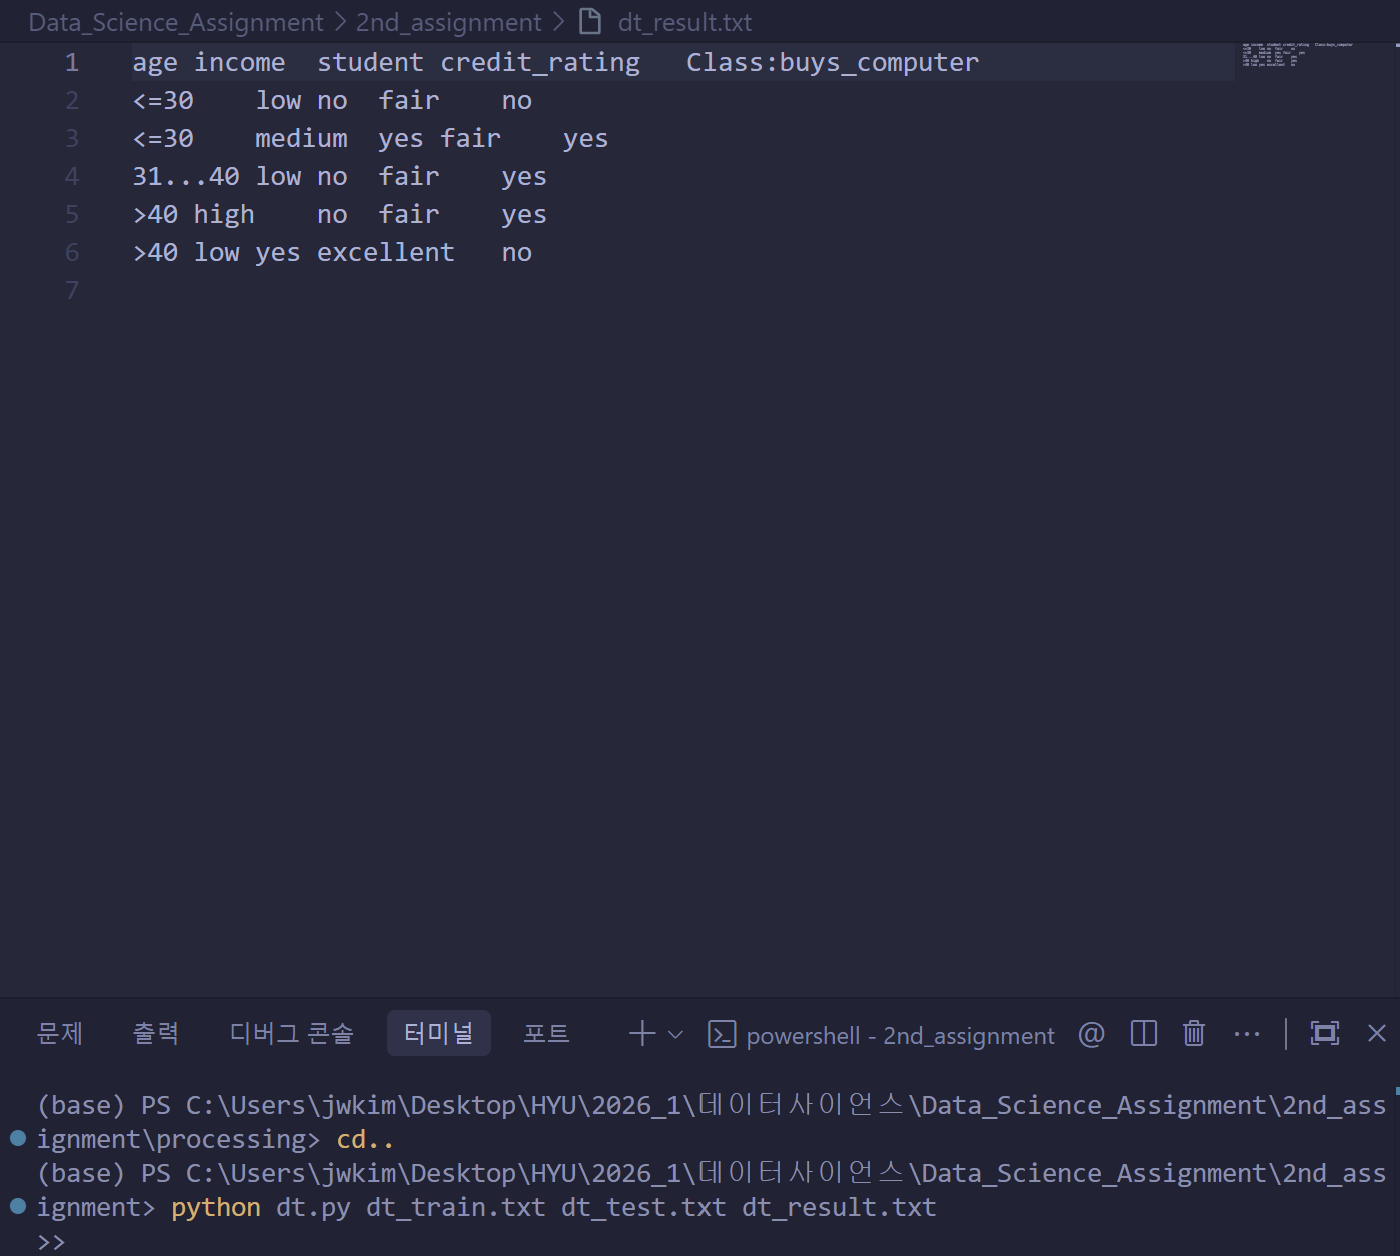
\includegraphics[width=0.9\textwidth]{screenshot.png}
\caption{터미널 환경에서의 과제 스크립트 구동 및 파일 생성 증빙 화면}
\end{figure}

정상적으로 처리 완료되면 터미널 상에서 별다른 에러 없이 즉시 종료되며, 요청한 출력 경로에 테스트 라벨이 도출된 \texttt{dt\_result.txt} 결과 파일이 탭(\texttt{\textbackslash t})으로 데이터가 구분되어 이상 없이 생성됩니다.

\end{document}
